%\chapter{Длинное название главы, в которой мы смотрим на примеры того, как будут верстаться изображения и списки} \label{chapt2}


\chapter{Определение позы камеры}

В данной главе я предлагаю метод определения позы камеры, основанный на анализе размеров изображений объектов интереса в наблюдаемой сцене. Предложенный метод имеет два ключевых отличия от предыдущих:
\begin{enumerate}
\item учитывает ложные обнаружения объектов интереса в сцене и неточности локализации присутствующих объектов;
\item предсказывает положение камеры даже при значительных углах её наклона.
\end{enumerate}

Позой камеры называется положение и направление съемки камеры относительно сцены. Таким образом, для определения позы камеры необходимо выбрать систему координат, связанную со сценой, называемую в дальнейшем мировой.

С камерой также связанна система координат. Для обозначения её базисных векторов в данной работе я использую $x_c$, $y_c$ и $z_c$. Начало координат камеры находится в её оптическом центре, $x_c$ совпадает с направлением вправо на изображении, а $y_c$ "--- с направлением вниз. Направление $z_c$ называется направлением камеры. Её положением является положение её оптического центра. Таким образом, поза камеры задает преобразование мировой системы координат в систему координат камеры.

Для дальнейшего описания предложенного метода следующем разделе я представляю модель наблюдаемых данных.

\section{Математическая модель наблюдаемых данных}  \label{chap-cam_pose::sec-model}

В данной работе я предлагаю модель наблюдаемых данных состоящих из плоской статичной сцены и людей, находящихся в ней. Такая аппроксимация подходит для описания большинства сценариев видеонаблюдения. Ниже я предлагаю описание трёх её составляющих моделей: сцены, камеры и человека.

\subsection{Модель сцены}

Под сценой в данной работе я подразумеваю неподвижные объекты, изображения которых получает камера. Таким образом сцена может состоять из дорог, зданий, деревьев, скамеек и др. Поскольку предлагаемый метод не использует семантическую информацию об объектах сцены, то в данной работе я рассматриваю простейшую модель сцены, состоящей из единственной горизонтальной плоскости "--- плоскости земли.

Для задания позы камеры необходимо выбрать мировую систему координат, связанную со сценой. Я использую $x_w$, $y_w$ и $z_w$ для обозначения её базисных векторов. Мировая система координат выбрана таким образом, что плоскость земли совпадает с плоскостью $z=0$, а вектор $z_w$ совпадает с направлением вверх в сцене. В качестве начала мировой системы координат я выбрал проекцию положения камеры на плоскость земли.

В данной работе я предполагаю, что скалярное произведение $y_c$ и $z_w$ отрицательно, т.е.~изображение не перевернуто, а вектор $x_w$ коллинеарен проекции вектора $z_c$ на плоскость земли. Описанные ограничения однозначно определяют мировую систему координат в наблюдаемой сцене.

\subsection{Модель камеры}

Я использую модель перспективной проекции, которая описывается фокусным расстоянием камеры $f_c$. Физические характеристики используемой камеры также описываются несколькими параметрами: размером матрицы камеры $w_c, h_c$, положением принципиальной точки $(x_c, y_c)$, размерами пикселя $(w_p, h_p)$ и углом его скоса $\alpha_c$. Я использую предположение камеры с квадратными пикселями ($w_p = y_p$, $\alpha_c$), принципиальная точка которой располагается в центре изображения ($x_c = \frac{w_c}{2}$, $y_c = \frac{h_c}{2}$).

При заданных ограничениях модель перспективная проекция полностью определяется матрицей внутренней калибровки камеры, которая имеет следующий вид:
\begin{equation}
	K = \left[
	\begin{matrix}
		f & 0 & w_I \\
		0 & f & h_I \\
		0 & 0 & 1
	\end{matrix} \right]
\end{equation},
где через $f = \frac{f_c}{w_p}$ "--- фокусное расстояние, вычисленное в размерах пикселя, а $(w_I, h_I)$ "--- размер изображения.

\subsection{Модель человека}

Единственными движущимися объектами в сцене являются люди. Я использовал модель человека, предложенную в статье \cite{pishchulin15arxiv}. Она является отображением параметров позы и комплекции в положение вершин трехмерной модели человека.

\section{Поза камеры}

Выбранная модель сцены однозначно определяет взаимное положение мировой системы координат и системы координат камеры. При заданных ограничениях поза камеры $l_{c}$ однозначно определяется тремя параметрами:
\begin{itemize}
	\item высотой $h$ камеры над плоскостью земли;
	\item углом $t$ наклона камеры;
	\item углом $r$ поворота камеры.
\end{itemize}

Высота $h$ камеры над плоскостью земли определяет положение оптического цента камеры на оси $z$. Углы наклона $t$ и поворота $r$ камеры являются углами нутации и собственного вращения при преобразовании мировой системы координат в систему координат камеры.

Формально задача определения позы камеры по изображению имеет следующий вид:
\begin{itemize}
\item[\textbf{Вход:}]
\begin{itemize}
\item Последовательность $\left\{I_t\right\}_t^T$ изображений, полученная статичной камерой;
\item Фокусное расстояние $f$ камеры;
\end{itemize}
\item[\textbf{Выход:}] Параметры позы камеры в сцене: $l_{c} = \left( h, t, r \right)$.
\end{itemize}

Алгоритм может быть использован для последовательностей, содержащих  как цветные, так и монохромные изображения произвольного размера. На наблюдаемые данные накладываются следующие ограничения:
\begin{itemize}
	\item в данный представлено не менее трех изображений людей, не расположенных на одной прямой;
	\item изображения голов людей имеют размер не менее $16\times16$ пикселей;
	\item высота $h$ камеры не превосходит 20 метров;
	\item угол поворота $r$ камеры находится в пределах $\left(-\frac{\pi}{12}, \frac{\pi}{12}\right)$;
	\item фокусное расстояние $f$ камеры ограничено $5000$ размерами пикселя.
\end{itemize}

Входная последовательность изображений может иметь произвольный размер, в частности содержать единственное изображение.

\section{Предложенный метод}

Я разработал метод определения позы камеры, основанный на анализе размеров изображений объектов интереса в наблюдаемой сцене. В качества объектов были выбраны головы людей, поскольку в отличие от фигур всего человека они меньше подвержены перекрытиям в сценарии видеонаблюдения.

Для построения отображения входного изображения в параметры камеры я использовал методы машинного обучения с учителем. В связи с отсутствием больших размеченных коллекций с известными положениями объектов и камеры в сцене обучение происходило на синтетической выборке.

\subsection{Построение обучающей выборки}

\begin{table} [htbp]
	\centering
	\caption{Распределение параметров позы камеры в синтетической выборке.}\label{tab:params}%
	%\begin{tabular}{|c|c|c|c|}
	\begin{tabulary}{\textwidth}{@{}>{\zz}L >{\zz}C >{\zz}C >{\zz}C}
		\hline
		Параметр & Название & Минимальное значение & Максимальное значение\\
		\hline
		\hline
		$h$ & высота (м) & 0 & 20 \\
		$t$ & наклон (рад) & $\frac{\pi}{2}$ & $\frac{11\pi}{12}$ \\
		$r$ & поворот (рад) & $-\frac{\pi}{12}$ & $\frac{\pi}{12}$ \\
		$f$ & фокусное расстояние (пиксели) & 0 & 5000 \\
		\hline
	\end{tabulary}
\end{table}

Обучающая выборка состоит из синтетических последовательностей изображений. Для её построения я использовал модель наблюдаемых данных, описанную в разделе \ref{chap-cam_pose::sec-model}. Параметры позы камеры выбирались из равномерного распределения с параметрами, представленными в таблице \ref{tab:params}

Алгоритм оценки позы камеры использует только положение и размер головы человека на изображение. Поэтому в синтетической выборке не моделируется разнообразие поз людей реального мира, и все люди находятся в стандартной позе. В качестве роста людей в сцене я выбрал 1.75 метра "--- средний рост взрослых европейцев.

При построении выборки изображения не удовлетворяющие ограничениям модели наблюдаемых данных отбраковывались. Построенная синтетическая выборка состоит из 100373 последовательностей, содержащих по 300 изображений в среднем. Каждое изображение содержит оного человека расположенного в произвольном месте изображения. Таким образом удается добиться того, что каждый человек хорошо виден на изображении.

\subsection{Выбор признакового описания}

Синтетические последовательности изображений визуально отличаются от реальных данных. Поэтому для обучения алгоритма регрессии позы необходимо выбрать признаковое описание инвариантное к используемой выборке.

В качестве описания я использую результаты обнаружения голов людей на изображении. Таким образом, каждый человек на изображении описывается тройкой чисел $\left(x_h, y_h, s_h\right)$, соответствующей положению центра его головы и её линейным размерам. Конечно, модель человека \cite{pishchulin2015building} позволяет определить реальное положение головы человека на синтетическом изображении. Однако, мы не можем применить тот же метод оценки положения головы человека к изображения реальных данных. Поэтому при использовании разных способов оценки положения головы человека на реальных и синтетических данных может возникнуть проблема оценки построенного алгоритма определения позы камеры. Поэтому я использовал метод локализации объектов на изображении даже к синтетическим данным. Такой подход позволил мне учесть небольшие ошибки в локализации и определении размеров алгоритмом локализации головы человека. Также этот подход позволяет использовать для определения позы камеры любые объекты, для которых доступна модель и алгоритм локализации на изображении.

Для локализации голов людей на изображении был выбран алгоритм \cite{prisacariu_reid_tr2310_09} и использована его оптимизированная версия \footnote{https://bitbucket.org/13e\_sha/fasterhog}. Использование данного алгоритма обусловлено высокой скоростью его работы. Этот фактор оказался очень важным для построения большой коллекции изображений синтетической выборки. Также данный алгоритм не чувствителен к наличию текстуры на изображении человека.

Для построения прецедента для обучения алгоритма регрессии позы камеры я использовал информацию о 64 людях в сцене. 

\subsection{Регрессия позы камеры}

Я использовал сверточную нейронную сеть для оценки позы камеры.

Важно отметить, что точность предсказания должна зависеть от позы камеры. При увеличении высоты камеры над плоскостью земли, точность её предсказания может уменьшаться. Таким образом, разные последовательности выборки могут иметь различную сложность при обучении.

Я учел это предположение в функции ошибки построенной нейронной сети. При решении задачи регрессии обычно используют Евклидову функцию потерь. К сожалению, она одинаково ``штрафует'' отклонение от правильного ответа для всех прецедентов. Для решения этой проблемы в качестве функции потерь я использовал взвешенную сумму квадратичных отклонений, где значение параметра и вес его вклада предсказывается нейронной сетью.

Формально, построенный алгоритм использует предположение нормального распределения позы камеры $l=\left( h, t, r \right)$ при условии наблюдаемых признаков сцены $x$ и  предсказывает математическое ожидание $\tilde{l_c}$ и дисперсию $\Sigma_c$ этого распределения: 
\begin{equation}
p(l_{c}|x, \Theta) = N(l_c|\tilde{l_c}(x, \Theta), \Sigma_c(x, \Theta))
\end{equation}

Матрица ковариации $\Sigma_c$ должна быть положительно определенной. Я учел это ограничение в функции потерь, добавив предположение о независимости параметров позы камеры. Также нейронная сеть предсказывает логарифм элементов матрицы ковариации:
\begin{equation}
	\Sigma_c(x, \Theta) = diag\left(e^{s(x, \Theta)}\right) + \epsilon I,
\end{equation}
где $s(x, \Theta) = \left( s_h(x, \Theta), s_t(x, \Theta), s_r(x, \Theta) \right)$ "--- вектор параметров матрицы ковариации. Параметр регуляризации $\epsilon$ был выбран равным $10^{-6}$.

Параметр $\lambda_c = \left|\Sigma_c^{-1}\right|$ можно интерпретировать как уверенность алгоритма в предсказании. Важно отметить, что в предложенном методе этот параметр зависит от наблюдаемых данных $x$.

В качестве функция потерь был выбран отрицательный логарифм правдоподобия наблюдаемых данных:
\begin{equation}
L(\left\{l_c\right\}_i | \left\{ \tilde{l_c^i} \right\}_i, \left\{s^i\right\}) = -\sum_i\log N(l_{c}^i|\tilde{l_c^i}, diag\left(e^{s^i}\right) + \epsilon I)
\label{eq:norm}
\end{equation}

\begin{figure*}[!t]
	\centering
	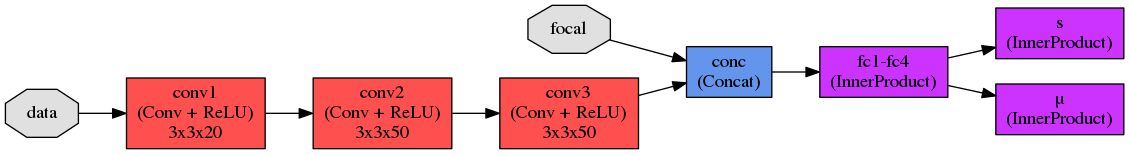
\includegraphics[width=\textwidth]{camera_pose/1}
	\caption{Схема использованной нейронной сети для предсказания параметров позы камеры.}
	\label{fig:net}
\end{figure*}

Производные используемой функции потерь могут быть вычислены аналитически:
\begin{align}
	\frac{\partial L}{\partial \tilde{\l_c^j}} &= 
	\frac{\tilde{\l_c^j} - l_c^j}{e^{s^j} + \epsilon}
	\label{eq:der_mu} \\
	\frac{\partial L}{\partial s^j} &= 
	\frac{1}{2}\frac{e^{s^j}}{e^{s^j} + \epsilon}
	\left(1 - \frac{(\tilde{l_c^j} - l_c^j) ^ 2}{e^{s^j} + \epsilon}\right)  \label{eq:der_sigma}
\end{align}

Выражения \eqref{eq:norm}, \eqref{eq:der_mu} и \eqref{eq:der_sigma} допускают эффективную реализацию используемой функции потерь на современных графических ускорителях.

Я использовал сверточную нейронную сеть прямого распространения. Входом нейронной сети является тензор размера $3\times8\times8$, описывающие положение и размер каждой из 64 обнаруженных голов. Чтобы алгоритму не потребовалось адаптироваться ко всевозможным перестановкам объектов прецедента, они были отсортированы по возрастанию размера.

Построенная нейронная сеть состоит из 3 сверточных слоёв, после которых используется нелинейная функция ReLu. Размер каждой сверки равер $3\times3$. Такой подход позволяет сверточным слоям 1) использовать информацию об удаленных объектах, размер которых существенно отличается и 2) адаптироваться к шуму в данных за счет использования объектов, чьи размеры отличаются слабо.

После применения сверточных слоёв полученный результат объединяется с фокусным расстоянием $f$ камеры и подается на вход полносвязным слоям. Описанная выше функция потерь позволяет обучать нейронную сеть предсказывать положение камеры и уверенность предсказания.

\subsection{Объединение результатов прецедентов}

Построенная нейронная сеть предсказывает позу камеры, используя положения не более 64 людей в сцене. Во реальных сценариях видеонаблюдения количество людей в сцене может существенно превышать это значение. Поэтому необходимо предложить метод объединения результатов на разных наборах данных.

Для решения этой проблемы можно объединить результаты работы алгоритма на $K$ разных подмножествах обнаружений людей с помощью наивного Байессовского метода:
\begin{align}
	\overline{l_c} &= \overline{\Sigma_c} \left( \sum_k^K{\Sigma_{c,k}^{-1} \tilde{l}_{c,k} } \right) \\
	\overline{\Sigma_c} &= \left( \sum_k^K \Sigma_{c,k}^{-1} \right) ^ {-1},
\end{align}
где $\overline{l_c}$ "--- предсказанная поза камеры.

Важно отметить, что данных подход может быть применен только при отсутствии зависимости между предсказанными позами камеры на разных подмножествах данных. Чтобы этого добиться, можно использовать непересекающиеся подмножества обнаружений объектов на разреженном подмножестве кадров.

To make the final solution we choose a distribution with the smallest differential entropy. For Gaussian distributions it also has the smallest determinant of the predicted covariance matrix $\Sigma$. The mean value of the chosen distribution is the predicted location of the camera. We show the chosen distribution in the second row of рисунка~\ref{fig:bestClear}. Рисунок~\ref{fig:TownCentre_calibration} presents synthesized people on the real image from the video sequence. We see that the presented and synthesized people have similar sizes. Thus the proposed model predicts plausible camera location. In further experiments we use the predicted camera height as the groundtruth.

\begin{figure*}[!t]
	\centering
	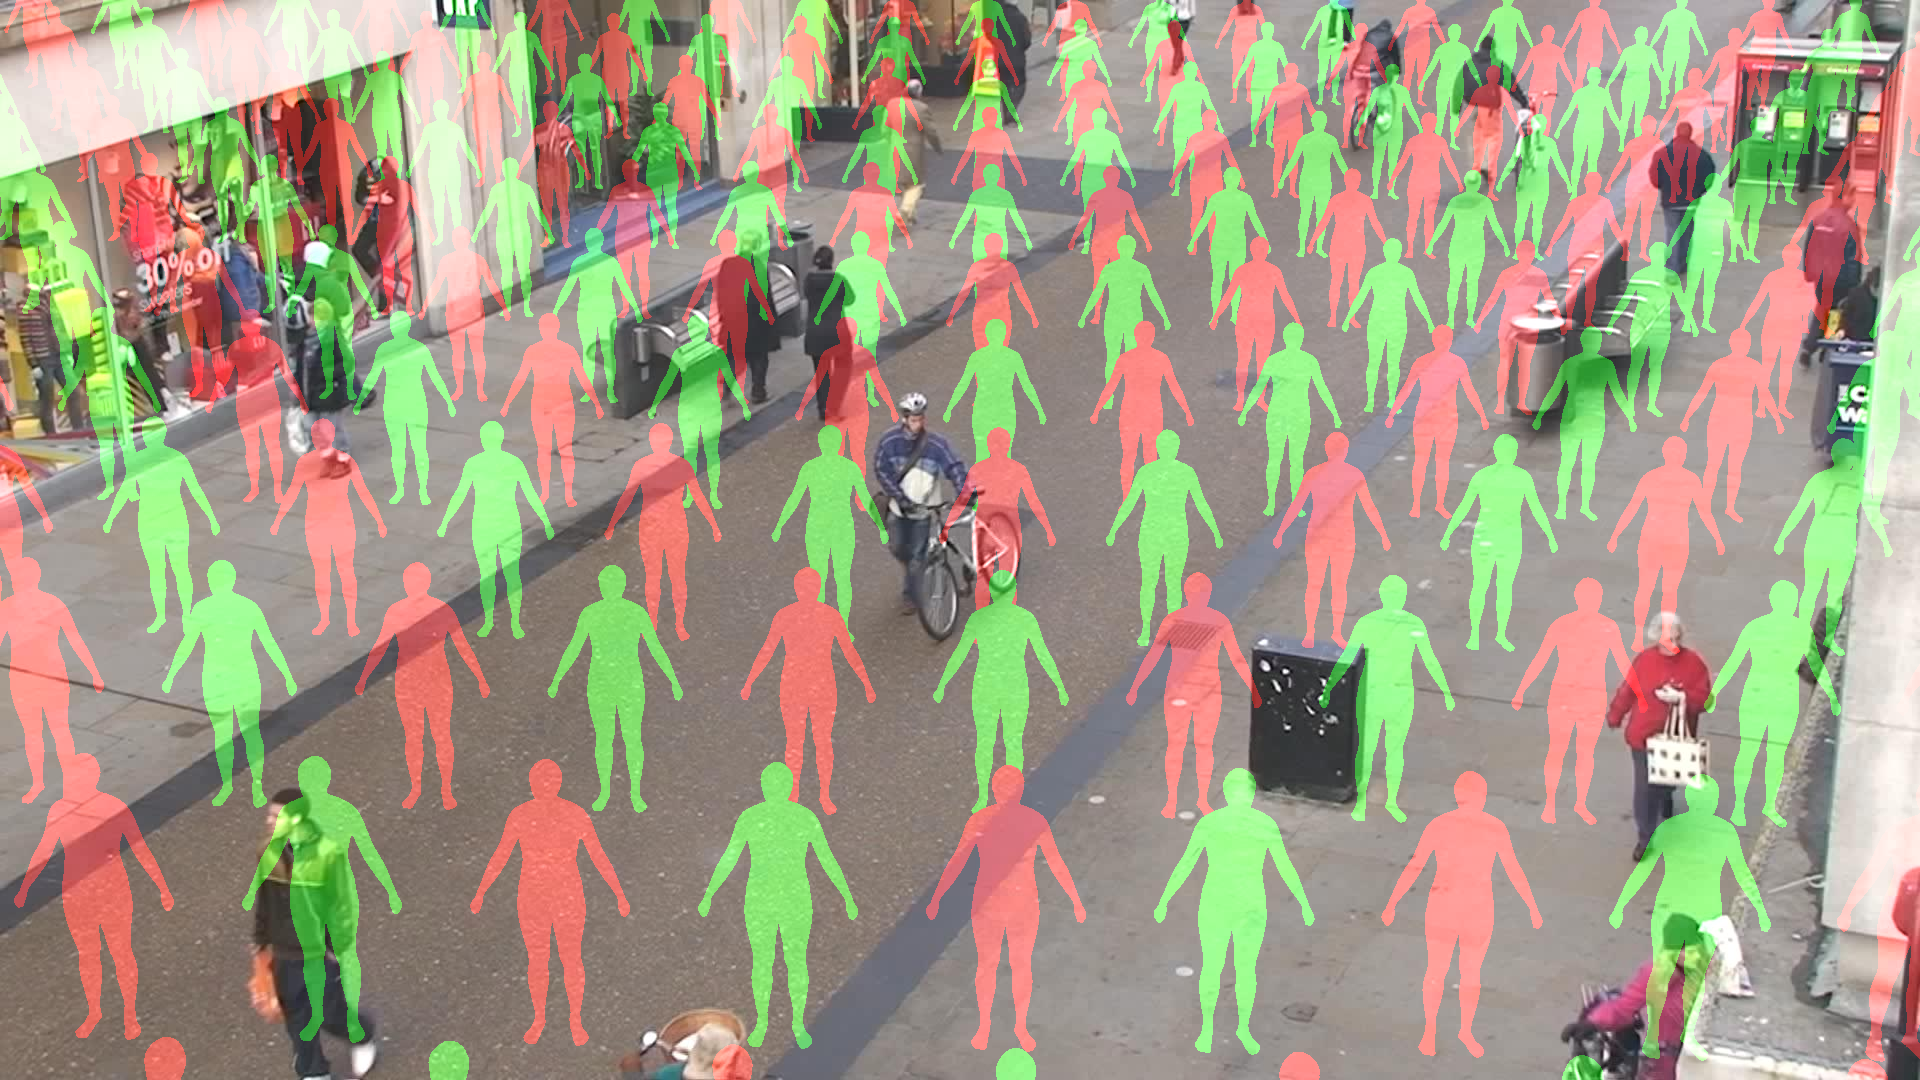
\includegraphics[height=72mm]{camera_pose/TownCentre_1}
	\caption{Визуализация синтезированных людей на предсказанной плоскости земли.}
	\label{fig:TownCentre_calibration}
\end{figure*}

In the next experiment we use all head detections on the TownCentre dataset. We repeat the proposed calibration technique used for clear detections. Note, that in average a number of false positives in the constructed samples are much higher than in train samples (52\% vs 10\%). The constructed results are shown in the third row of \ref{fig:bestClear}. It shows that the predicted camera location is close to its true value even when there are a huge number of false positive detections.

In addition we experiment with duplicate detections in a sample. We choose a single true positive head found by the detector and construct a sample that contains 64 copies of this head. Such an extreme case of duplication corresponds to a scene with a single person standing in the same place for a long time. Camera location cannot be predicted from this sample as is it specifies only distance to the single person in a scene. Рисунок~\ref{fig:bestClear} shows that the model predicts a very significant error for camera locations that can produce such a detection. Thus a determinant of the predicted covariance matrix is a good measure of the model confidence.

Our training data assumes that people can be found in each location of the input images. Thus, each training sample contains people uniformly distributed in the image plane. Hence, the long input video sequence is preferable as it gives better statistics of people sizes across image plane.

We evaluate the proposed method on four video sequences of the more challenging PETS 2006 dataset \cite{thirde2006overview}. It's important to notice, that the first and second video sequences of this dataset violate our assumption of a single ground plane. These video sequences contain people on several floors. Nevertheless, we apply the proposed method to all video sequences in the dataset and use all detector results as the features. Our evaluation (см. таблица~\ref{tab:PETS}) reveals that the proposed method correctly estimate camera location on the third and fourth sequence and cannot predict plausible camera pose on the first two sequences. However the predicted deviation is significantly larger for such failure cases, thus the model indicates low confidence in these predictions.

\section{Обучение и экспериментальная оценка}

В этом разделе я опишу используемый метод обучения параметров построенного алгоритма и результаты его тестирования на синтетических и реальных данных.

\subsection{Обучение}

Обучение нейронной сети проводилось на построенной синтетической выборке. Данная выборка содержит только верные обнаружения голов людей. Эксперименты показали, что обучение на таких ``чистых'' данных не позволяет алгоритму обобщаться на обнаружения, содержащие ошибки.

Для решения этой проблемы я промоделировал два типа шума в реальных данных: 1) ложные обнаружения голов в сцене; 2) дублирующиеся обнаружения в прецеденте. Второй тип шума может возникать, если человек неподвижен на нескольких кадрах. Для моделирования шума был применен следующий алгоритм:
\begin{enumerate}
	\item из множества обнаружений последовательности выбиралось подмножество из $n: 0 < n \le 64$ элементов;
	\item среди выбранных обнаружений $m: 0 < m < \frac{n}{10}$ произвольных заменялись на ложные срабатывания детектора со случайным положением и размером в сцене;
	\item из построенного множества производилась выборка 64 обнаружений с повторениями.
\end{enumerate}

Такой подход позволил промоделировать ложные срабатывания алгоритма локализации людей и дублирование обнаружений на разных кадрах. По каждой последовательности обучающей выборки было построено 3 прецедента.

Предложенная сверточная нейронная сеть имеет всего 67393 параметра и относительно небольшие размеры промежуточных слоёв. Это позволило сформировать батчи состоящие из 32768 прецедентов при обучении с помощью градиентного спуска. Скорость обучения понижалась по степенному закону с параметром $\gamma=0.95$ каждые 1500 итераций. Обучение заняло 200000 итераций. Я использовал 80\% последовательностей синтетической выборки для обучения и 20\% для валидации.

Важно отметить, что из-за использования алгоритма локализации объектов на изображении, обученные параметры нейронной сети чувствительны к смене алгоритма локализации объектов. Таким образом, при его замене необходимо повторное обучение.  С другой стороны, предложенный подход позволяет отказаться от моделирования неточностей в локализации объектов используемым алгоритмом. Более того, при его замене обученные параметры нейронной сети могут являться хорошим начальным приближением.

\subsection{Экспериментальная оценка на синтетической выборке}

Я провел несколько экспериментов для оценить качество построенного алгоритма. 

Первый эксперимент показывает влияние размера обучающей выборки и архитектуры нейронной сети на качество построенного регрессора. Я провел тестирование нейронных сетей с разным количеством полносвязных слоёв (см.~таблицу \ref{part2::arch_quality}). Среднеквадратичная ошибка регрессора на валидационной выборке оказывается неинформативной мерой качества алгоритма, так как размерности и диапазоны значений параметров позы камеры различаются. Для решения этой проблемы я использовал $L_1$ расстояние между предсказанными и верными параметрами, нормализованными на диапазон их значений в обучающей выборке (см.~таблицу \ref{tab:params}). Результаты сравнения показали, что увеличение размера обучающей выборки и количество полносвязных слоёв приводит к повышению точности определения позы камеры. Наилучших результатов удается добиться при обучении нейронной сети, содержащей 5 полносвязных слоёв, на обучающей выборке из 80298 сцен. Также тестирование показало, что при выбранных параметрах не происходит переобучение алгоритма к обучающим данным, так как ошибки на обучающей и валидационной выборках близки.

\begin{table} [htbp]
	\caption{Зависимость нормализованного отклонения на обучающей и валидационной выборках.}\label{part2::arch_quality}%
	\begin{tabulary}{\textwidth}{@{}>{\zz}L >{\zz}C >{\zz}C >{\zz}C}
		\hline
		Размер выборки (последовательностей) & Количество полносвязных слоёв & Средняя ошибка на обучении & Средняя ошибка на валидации\\
		\hline
		20448 & 3 & 0.1061 & 0.121 \\
		20448 & 4 & 0.0956 & 0.1167 \\
		20448 & 5 & 0.07 & 0.12 \\
		30179 & 4 & 0.09015 & 0.117 \\
		51366 & 4 & 0.09836 & 0.1064 \\
		80298 & 5 & 0.09764 & \textbf{0.1009} \\
		\hline
	\end{tabulary}
\end{table}

\subsection{Экспериментальная оценка на реальных данных}

\begin{figure*}[ht]
	\centering
	\begin{tabular}{ccc}
		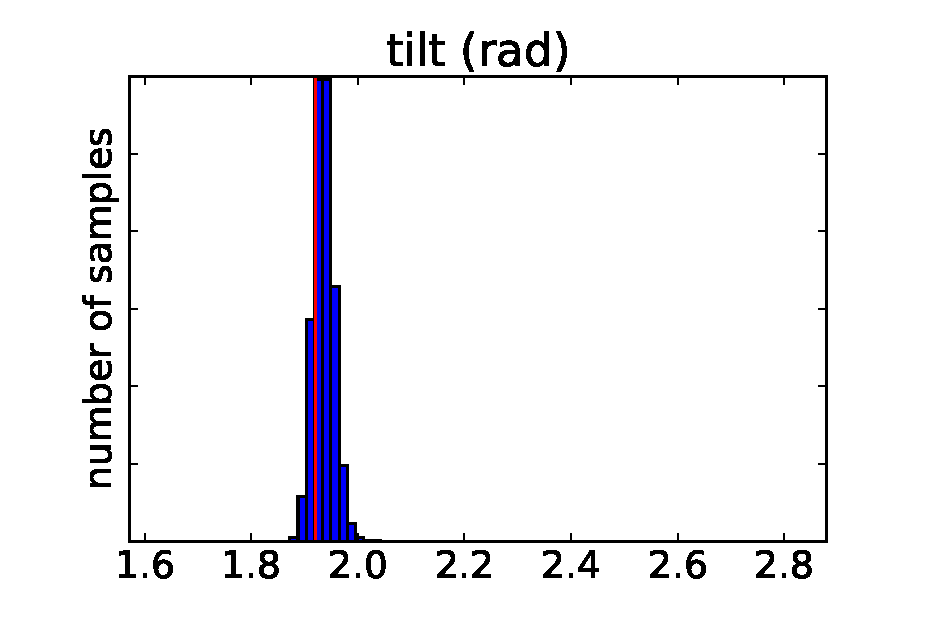
\includegraphics[height=26mm]{camera_pose/clear_detections_tilt} &
		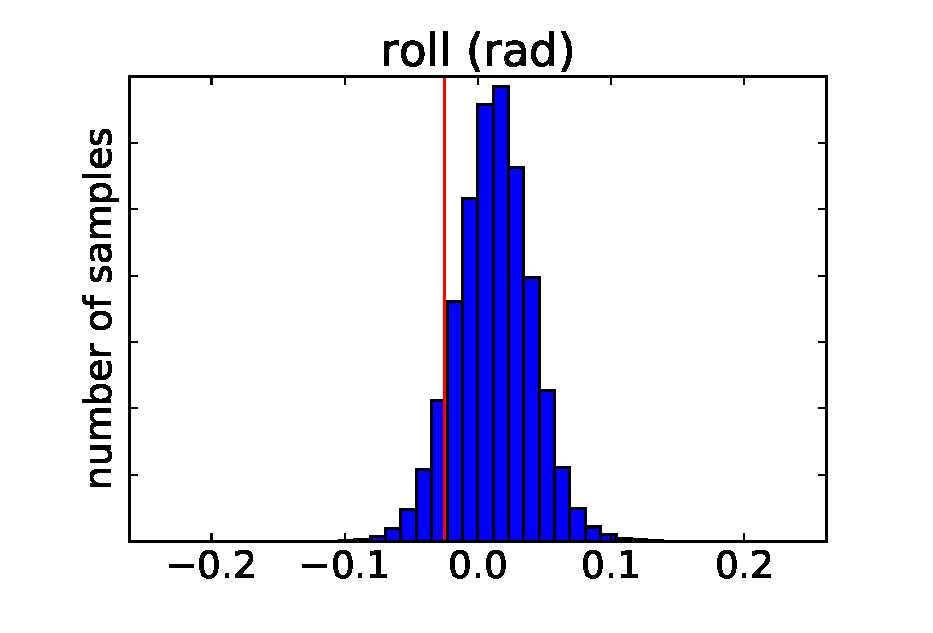
\includegraphics[height=26mm]{camera_pose/clear_detections_roll} &
		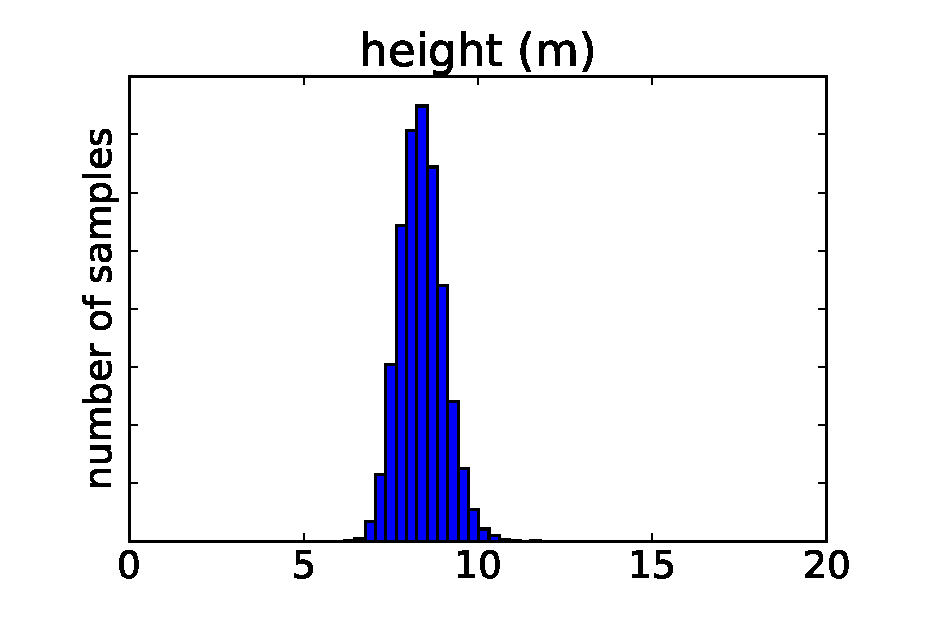
\includegraphics[height=26mm]{camera_pose/clear_detections_height} \\
		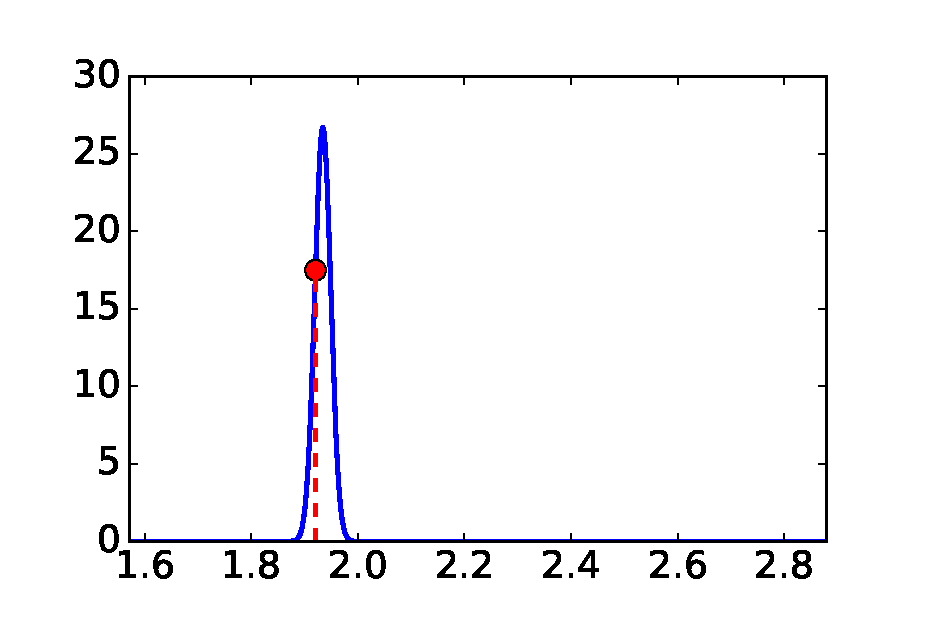
\includegraphics[height=26mm]{camera_pose/bestClear_0} &
		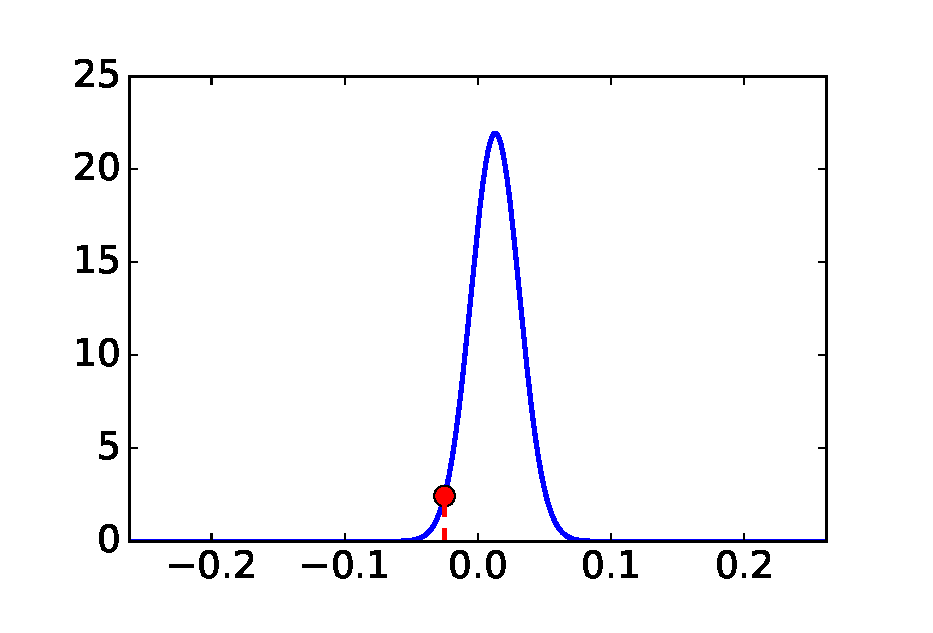
\includegraphics[height=26mm]{camera_pose/bestClear_1} &
		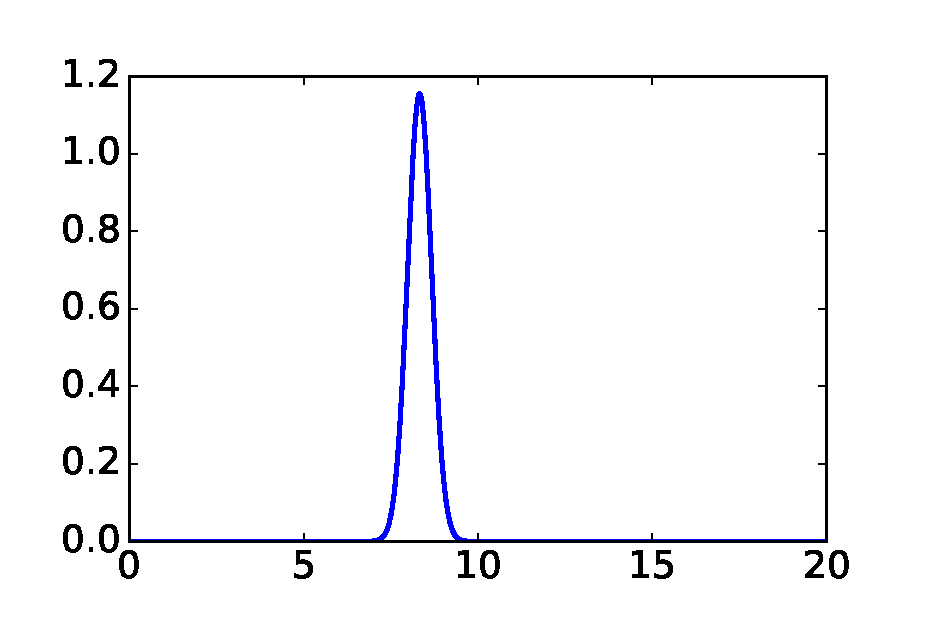
\includegraphics[height=26mm]{camera_pose/bestClear_2} \\
		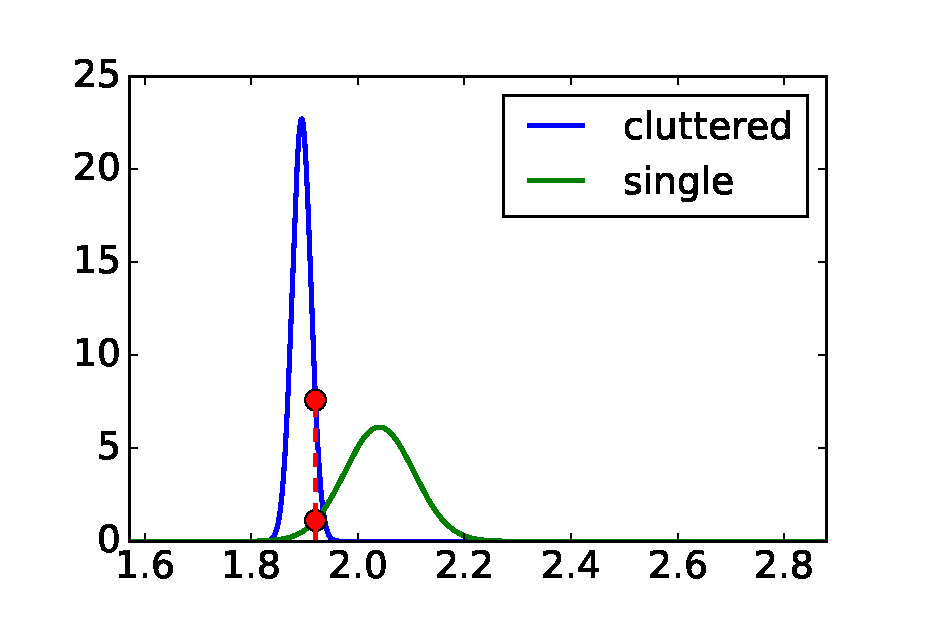
\includegraphics[height=26mm]{camera_pose/combinedObservations_0} &
		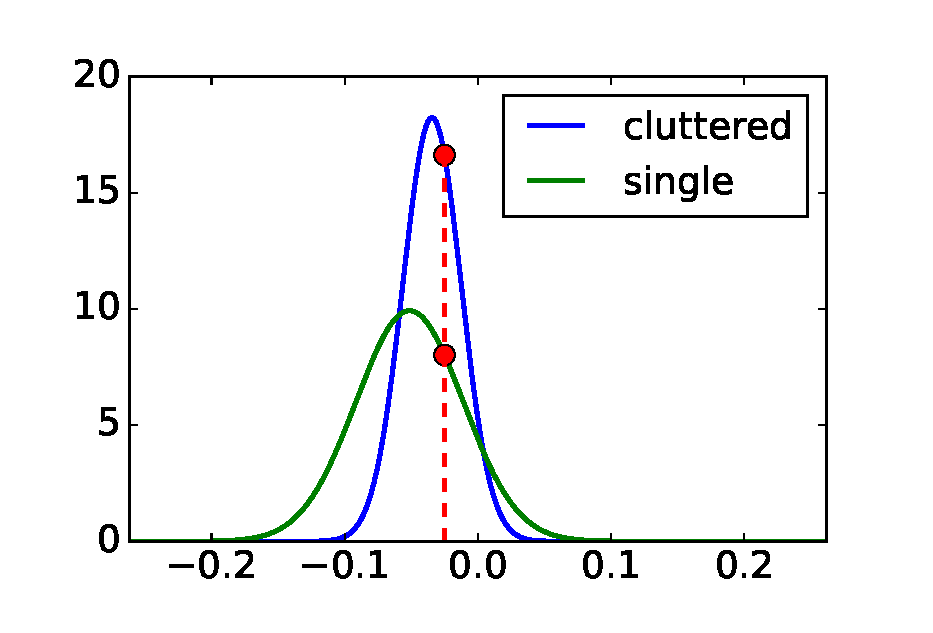
\includegraphics[height=26mm]{camera_pose/combinedObservations_1} &
		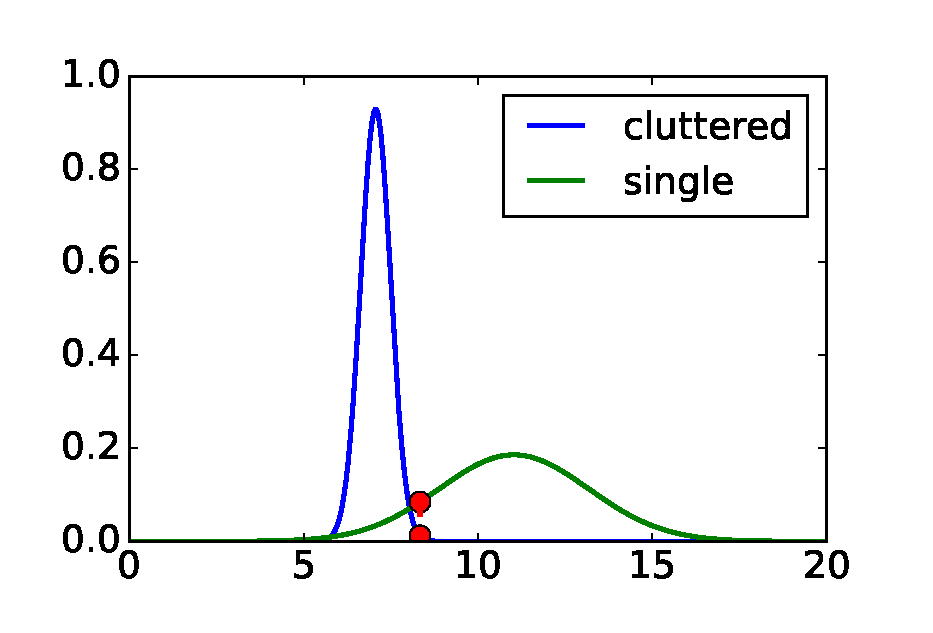
\includegraphics[height=26mm]{camera_pose/combinedObservations_2} \\
	\end{tabular}
	\caption{Результаты определения позы камеры на выборке TownCentre. В первой строке представлены гистограммы предсказанных параметров камеры на разных подмножествах верных обнаружений людей в выборке (голубым). Во второй строке указано предсказанное распределение положения камеры. В третьей строке представлено предсказанное распределение положения камеры на данных, содержащих ложно-положительные обнаружения, (синий) и единственное верное обнаружение (зеленый). Параметры позы камеры, представленные в экспертной разметке, отмеченны красным. Столбцы соответствуют углам наклона и поворота и высоте камеры над плоскостью земли.}
	\label{fig:bestClear}
\end{figure*}

\begin{table*}[t] 
	\begin{center}
		\captionsetup{width=15cm}		
		\caption{Предсказанные параметры положения камеры на выборке TownCentre для <<чистых>>, <<зашумленных>> данных и данных, содержащих единственное обнаружение головы. Таблица содержит предсказанные параметры позы камеры и их среднеквадратичные отклонения.} \label{tab:symbols}
		\begin{tabular}{|c|c|c|c|} 
			\hline
			& Наклон & Поворот & Высота \\ \hline \hline
			экспертная разметка & $1.9205$ & $-0.0251$ & --- \\
			``чистые'' данные & $1.9342 \pm 0.0149$ &
			$0.0130 \pm 0.0182$ &
			$8.3290 \pm 0.3453$ \\
			``зашумлённые'' данные & $1.8945 \pm 0.0176$ &
			$-0.0345 \pm 0.0219$ &
			$7.0696 \pm 0.4294$ \\
			единственное обнаружение & $2.0402 \pm 0.0649$ &
			$-0.0513 \pm 0.0402$ &
			$11.0312 \pm 2.1441$ \\ \hline
		\end{tabular}
	\end{center}
\end{table*}

Предложенный алгоритм был протестирован на нескольких доступных выборках. В качестве первого эксперимента была использована выборка TownCentre \cite{benfold2011stable}, так как она содержит экспертную разметку положения голов людей и калибровки камеры. Однако, мне не удалось использовать указанное значение высоты камеры над уровнем земли, так как не указаны используемые единицы измерения длины.

Я применил алгоритм детектирования голов людей на изображении fastHOG \cite{prisacariu2009fasthog} к каждому кадру выборки. Те обнаружения, чьё пересечение с результатами экспертной разметки превосходило значение 0.5 по метрике IoU, рассматривались в качестве верных обнаружений. При таком выборе точность алгоритма составляла 48\%, и было обнаружено 19061 головы человека на 4501 кадре. Из них было случайным образом выбрано 40000 прецедентов, содержащие по 64 обнаружения с повторениями. В первой строке рисунка~\ref{fig:bestClear} показаны распределения ответов на разных прецедентах. Можно заметить, что указанные распределения имеют явно выраженную моду близкую к правильному значению параметров.

Для выбора позы камеры я протестировал две стратегии: 1) выбор предсказания с наибольшим значением уверенности $\lambda$; 2) выбор объединения предсказаний в рамках наивного байессовского подхода. В рамках второго подхода было случайно выбрано 20 прецедентов, множества обнаружений которых не пересекаются. Такой подход обеспечивает большую независимость результатов работы алгоритма на разных прецедентах. Во второй строке рисунка~\ref{fig:bestClear} представлены предсказания позы камеры для разных стратегий. Можно заметить, что в данной последовательности значения предсказаний отличаются слабо. Однако первая стратегия может приводить к неверным результатам, так как значение уверенности $\lambda$ меньше, когда значения параметров предсказанной позы близко к границе допустимых значений.

На рисунке~\ref{fig:TownCentre_calibration} представлена визуализация синтезированных людей на плоскости земли при предсказанной позе камеры. Можно заметить, что размеры реальных и синтезированных людей похожи, что подтверждает правдоподобие предсказанной позы камеры, поэтому в последующих экспериментах с выборкой TownCentre я использую предсказанную высоту камеры над плоскостью земли в качестве экспертной разметки.

\begin{figure*}[!t]
	\centering
	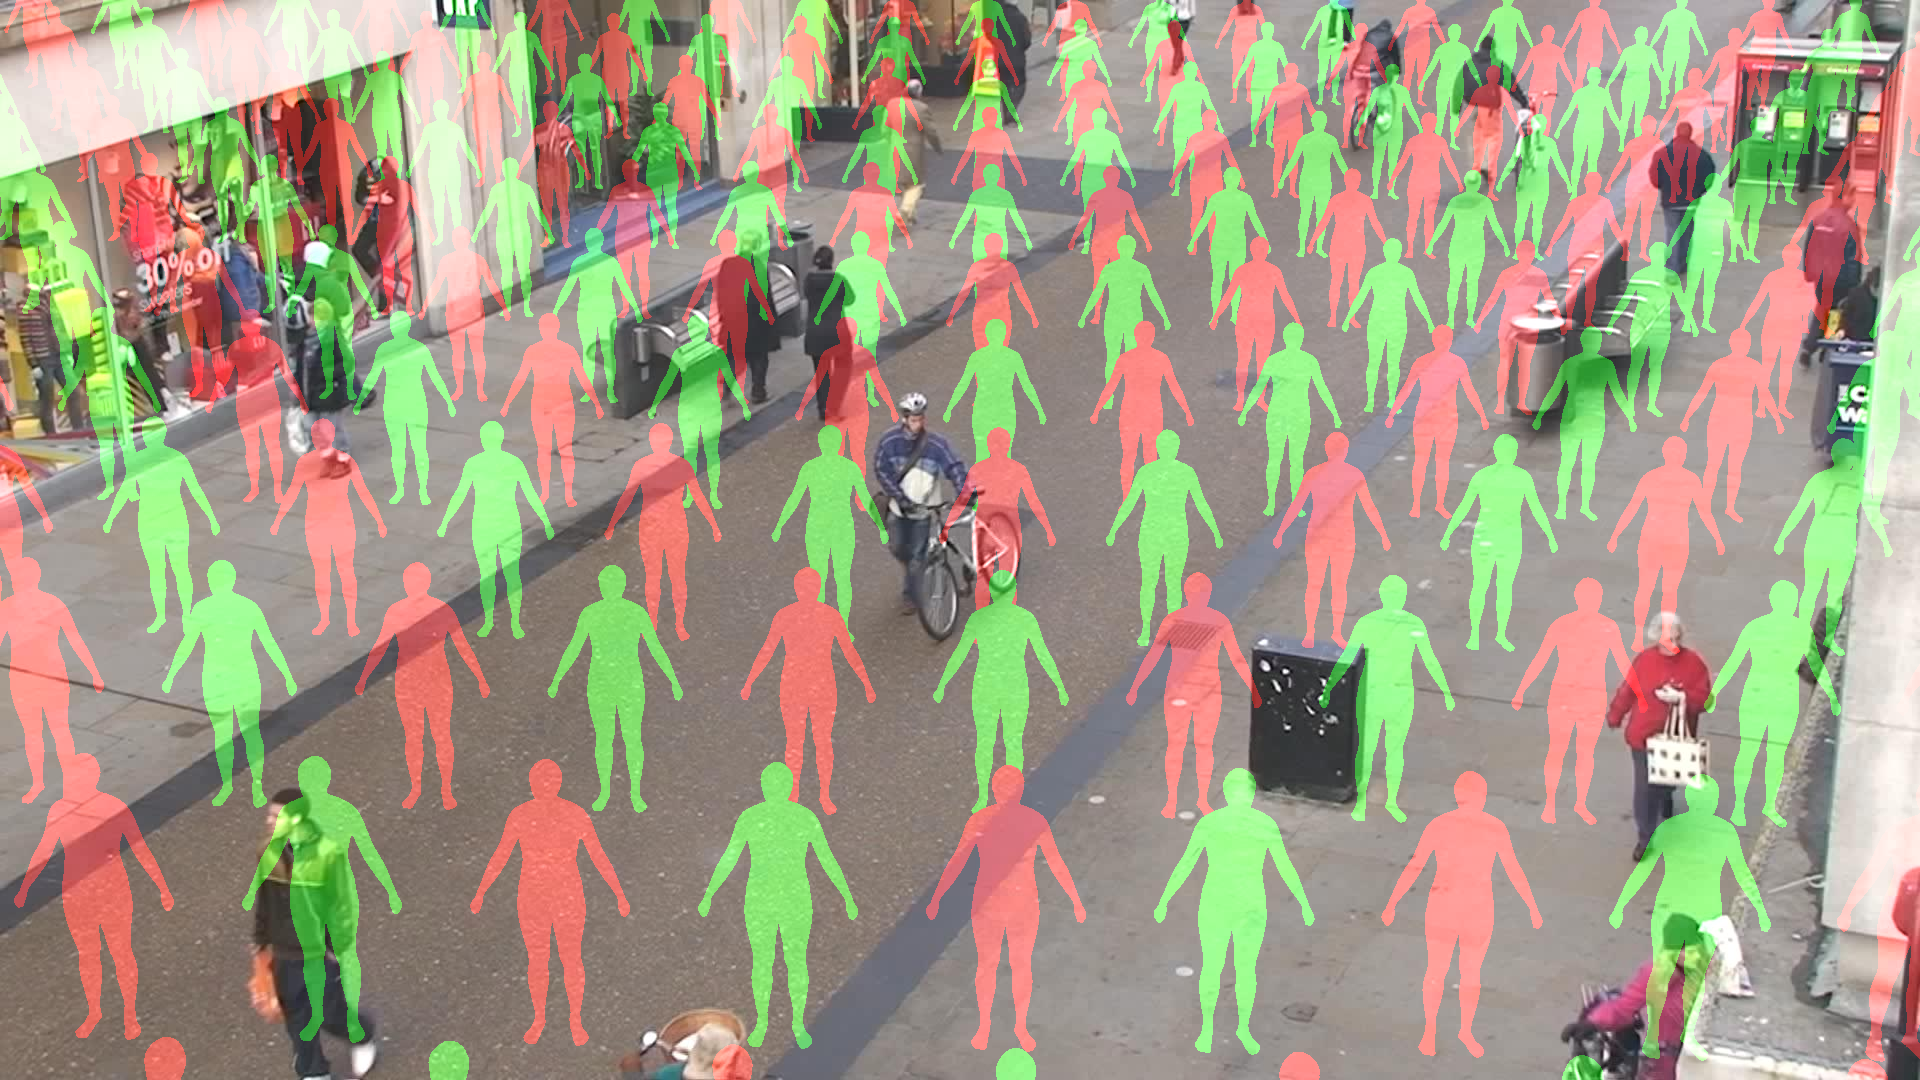
\includegraphics[height=72mm]{camera_pose/TownCentre_1}
	\caption{Визуализация синтезированных людей на предсказанной плоскости земли.}
	\label{fig:TownCentre_calibration}
\end{figure*}

В следующем эксперименте я использовал все обнаружения на выборке TownCentre. Я повторил предложенный метод калибровки
In the next experiment we use all head detections on the TownCentre dataset. We repeat the proposed calibration technique used for clear detections. Note, that in average a number of false positives in the constructed samples are much higher than in train samples (52\% vs 10\%). The constructed results are shown in the third row of \ref{fig:bestClear}. It shows that the predicted camera location is close to its true value even when there are a huge number of false positive detections.

In addition we experiment with duplicate detections in a sample. We choose a single true positive head found by the detector and construct a sample that contains 64 copies of this head. Such an extreme case of duplication corresponds to a scene with a single person standing in the same place for a long time. Camera location cannot be predicted from this sample as is it specifies only distance to the single person in a scene. Рисунок~\ref{fig:bestClear} shows that the model predicts a very significant error for camera locations that can produce such a detection. Thus a determinant of the predicted covariance matrix is a good measure of the model confidence.

Our training data assumes that people can be found in each location of the input images. Thus, each training sample contains people uniformly distributed in the image plane. Hence, the long input video sequence is preferable as it gives better statistics of people sizes across image plane.

We evaluate the proposed method on four video sequences of the more challenging PETS 2006 dataset \cite{thirde2006overview}. It's important to notice, that the first and second video sequences of this dataset violate our assumption of a single ground plane. These video sequences contain people on several floors. Nevertheless, we apply the proposed method to all video sequences in the dataset and use all detector results as the features. Our evaluation (см. таблица~\ref{tab:PETS}) reveals that the proposed method correctly estimate camera location on the third and fourth sequence and cannot predict plausible camera pose on the first two sequences. However the predicted deviation is significantly larger for such failure cases, thus the model indicates low confidence in these predictions.


\begin{table*}[t] 
	\begin{center}
		\captionsetup{width=15cm}
		\caption{Предсказанные параметры позы камеры на выборке PETS 2006. Таблица содержит предсказанные параметры позы камеры и их среднеквадратичные отклонения.} \label{tab:PETS}
		\begin{tabular}{|c|c|c|c|c|} 
			\hline
			последовательность & & Наклон & Поворот & Высота \\ \hline \hline
			\multirow{2}{*}{PETS 1} & верное & $1.6758$ & $-0.0172$ & $1.8786$  \\
			& оцененное & $2.0166 \pm 0.0612$ & $-0.0012 \pm 0.0356$ &  $4.5958 \pm 0.8783$ \\ \hline
			\multirow{2}{*}{PETS 2} & верное & $1.5346$ & $-0.0959$ & $4.6097$  \\
			& оцененное & $1.7315 \pm 0.0715$ & $-0.0374 \pm 0.0428$ &  $9.377 \pm 1.0811$ \\ \hline
			\multirow{2}{*}{PETS 3} & верное & $1.86$ & $-0.0304$ & $5.5016$ \\
			& оцененное & $1.9287 \pm 0.0241$ & $-0.0246 \pm 0.0225$ &  $5.8238 \pm 0.2988$ \\ \hline
			\multirow{2}{*}{PETS 4} & верное & $2.0290$ & $-0.1095$ & $6.5672$ \\
			& оцененное & $2.0247 \pm 0.0249$ & $0.059 \pm 0.0236$ & $5.3678 \pm 0.3262$ \\ \hline
		\end{tabular}
	\end{center}
\end{table*}

\section{Одиночное изображение} \label{sect2_1}

\begin{figure}[ht] 
  \center
  \includegraphics [scale=0.27] {latex}
  \caption{TeX.} 
  \label{img:latex}  
\end{figure}

%\newpage
%============================================================================================================================
\section{Длинное название параграфа, в котором мы узнаём как сделать две картинки с общим номером и названием} \label{sect2_2}

А это две картинки под общим номером и названием:
\begin{figure}[ht]
  \begin{minipage}[ht]{0.49\linewidth}
    \center{\includegraphics[width=0.5\linewidth]{knuth1} \\ а)}
  \end{minipage}
  \hfill
  \begin{minipage}[ht]{0.49\linewidth}
    \center{\includegraphics[width=0.5\linewidth]{knuth2} \\ б)}
  \end{minipage}
  \caption{Очень длинная подпись к изображению, на котором представлены две фотографии Дональда Кнута}
  \label{img:knuth}  
\end{figure}

Те~же~две картинки под~общим номером и~названием, но с автоматизированной нумерацей подрисунков посредством пакета \verb|subcaption|:
\begin{figure}[ht]
    \center{
        \hfill
        \subcaptionbox[List-of-Figures entry]{Первый подрисунок\label{img:knuth_2_1}} {\includegraphics[width=0.25\linewidth]{knuth1}}%
        \hfill       
        \subcaptionbox{Второй подрисунок\label{img:knuth_2_2}} {\includegraphics[width=0.25\linewidth]{knuth2}}
        \hfill
    }

    Подрисуночный текст, описывающий обозначения, например. Согласно ГОСТ 2.105, пункт 4.3.1, располагается перед наименованием рисунка.
    \caption{Очень длинная подпись к второму изображению, на котором представлены две фотографии Дональда Кнута} % Этот текст попадает в названия рисунков в списке рисунков
    \label{img:knuth_2}
\end{figure}


На рисунке~\ref{img:knuth_2_1} показан Дональд Кнут без головного убора. На рисунке~\ref{img:knuth_2}\subref*{img:knuth_2_2}  показан Дональд Кнут в головном уборе.

%\newpage
%============================================================================================================================
\section{Пример вёрстки списков} \label{sect2_3}

\noindent Нумерованный список:
\begin{enumerate}
  \item Первый пункт.
  \item Второй пункт.
  \item Третий пункт.
\end{enumerate}

\noindent Маркированный список:
\begin{itemize}
  \item Первый пункт.
  \item Второй пункт.
  \item Третий пункт.
\end{itemize}

\noindent Вложенные списки:
\begin{itemize}
  \item Имеется маркированный список.
  \begin{enumerate}
    \item В нём лежит нумерованный список,
    \item в котором
    \begin{itemize}
      \item лежит ещё один маркированный список.
    \end{itemize}    
  \end{enumerate}
\end{itemize}


\section{Пробелы}

В~русском наборе принято:
\begin{itemize}
    \item единицы измерения, знак процента отделять пробелами от~числа: 10~кВт, 15~\% (согласно ГОСТ 8.417, раздел 8);
    \item $\tg 20^\circ$, но: 20~${}^\circ$C (согласно ГОСТ 8.417, раздел 8);
    \item знак номера, параграфа отделять от~числа: №~5, \S~8;
    \item стандартные сокращения: т.\:е., и~т.\:д., и~т.\:п.;
    \item неразрывные пробелы в~предложениях.
\end{itemize}

\section{Математика}

Русская традиция начертания греческих букв отличается от~западной. Это исправляется серией \verb|\renewcommand|.
\begin{itemize}
    \item[До:] $ \epsilon \ge \phi$, $\phi \leq \epsilon$, $\kappa \in \emptyset$.
    \renewcommand{\epsilon}{\ensuremath{\varepsilon}}
    \renewcommand{\phi}{\ensuremath{\varphi}}
    \renewcommand{\kappa}{\ensuremath{\varkappa}}
    \renewcommand{\le}{\ensuremath{\leqslant}}
    \renewcommand{\leq}{\ensuremath{\leqslant}}
    \renewcommand{\ge}{\ensuremath{\geqslant}}
    \renewcommand{\geq}{\ensuremath{\geqslant}}
    \renewcommand{\emptyset}{\varnothing}
    \item[После:] $\epsilon \ge \phi$, $\phi \leq \epsilon$, $\kappa \in \emptyset$.
\end{itemize}

Кроме того, принято набирать греческие буквы вертикальными, что решается подключением пакета \verb|upgreek| (см. закомментированный блок в \verb|userpackages.tex|) и~аналогичным переопределением в преамбуле (см. закомментированный блок в \verb|userstyles.tex|).


\section{Кавычки}
В английском языке приняты одинарные и двойные кавычки в~виде ‘...’ и~“...”. В России приняты французские («...») и~немецкие („...“) кавычки (они называются «ёлочки» и~«лапки», соответственно). <<Лапки>> обычно используются внутри ,,ёлочек``, например, <<... наш гордый ,,Варяг``...>>.

Французкие левые и правые кавычки набираются
как лигатуры \verb|<<| и \verb|>>|, а~немецкие левые и правые кавычки набираются как лигатуры \verb|,,| и \verb|‘‘| (\verb|``|).

Вместо лигатур или команд с~активным символом "\ можно использовать команды \verb|\glqq| и \verb|\grqq| для набора немецких кавычек и команды \verb|\flqq| и \verb|\frqq| для набора французских кавычек. Они определены в пакете \verb|babel|.

\section{Тире}
%  babel+pdflatex по умолчанию, в polyglossia надо включать опцией (и перекомпилировать с удалением временных файлов)
Команда \verb|"---| используется для печати тире в тексте. Оно несколько короче английского длинного тире. Кроме того, команда задаёт небольшую жёсткую отбивку от слова, стоящего перед тире. При этом, само тире не отрывается от слова. После тире следует такая же отбивка от текста, как и перед тире. При наборе текста между словом и командой, за которым она следует, должен стоять пробел.

В составных словах, таких, как <<Закон Менделеева"--~Клапейрона>>, для печати тире надо использовать команду \verb|"--~|. Она ставит более короткое, по~сравнению с~английским, тире и позволяет делать переносы во втором слове. При~наборе текста команда \verb|"--~| не отделяется пробелом от слова, за которым она следует (\verb|Менделеева"--~|). Следующее за командой слово может быть  отделено от~неё пробелом или перенесено на другую строку.

Если прямая речь начинается с~абзаца, то перед началом её печатается тире командой
\verb|"--*|. Она печатает русское тире и жёсткую отбивку нужной величины перед текстом.

\section{Дефисы и переносы слов}
%  babel+pdflatex по умолчанию, в polyglossia надо включать опцией (и перекомпилировать с удалением временных файлов)
Для печати дефиса в~составных словах введены две команды. Команда~\verb|"~| печатает дефис и~запрещает делать переносы в~самих словах, а~команда \verb|"=| печатает дефис, оставляя \TeX ’у право делать переносы в~самих словах.

В отличие от команды \verb|\-|, команда \verb|"-| задаёт место в~слове, где можно делать перенос, не~запрещая переносы и~в~других местах слова.

Команда \verb|""| задаёт место в~слове, где можно делать перенос, причём дефис при~переносе в~этом месте не~ставится.

Команда \verb|",| вставляет небольшой пробел после инициалов с~правом переноса в~фамилии.

\section{Текст из панграмм и формул}

Любя, съешь щипцы, "--- вздохнёт мэр, "--- кайф жгуч. Шеф взъярён тчк щипцы с~эхом гудбай Жюль. Эй, жлоб! Где туз? Прячь юных съёмщиц в~шкаф. Экс-граф? Плюш изъят. Бьём чуждый цен хвощ! Эх, чужак! Общий съём цен шляп (юфть) "--- вдрызг! Любя, съешь щипцы, "--- вздохнёт мэр, "--- кайф жгуч. Шеф взъярён тчк щипцы с~эхом гудбай Жюль. Эй, жлоб! Где туз? Прячь юных съёмщиц в~шкаф. Экс-граф? Плюш изъят. Бьём чуждый цен хвощ! Эх, чужак! Общий съём цен шляп (юфть) "--- вдрызг! Любя, съешь щипцы, "--- вздохнёт мэр, "--- кайф жгуч. Шеф взъярён тчк щипцы с~эхом гудбай Жюль. Эй, жлоб! Где туз? Прячь юных съёмщиц в~шкаф. Экс-граф? Плюш изъят. Бьём чуждый цен хвощ! Эх, чужак! Общий съём цен шляп (юфть) "--- вдрызг! Любя, съешь щипцы, "--- вздохнёт мэр, "--- кайф жгуч. Шеф взъярён тчк щипцы с~эхом гудбай Жюль. Эй, жлоб! Где туз? Прячь юных съёмщиц в~шкаф. Экс-граф? Плюш изъят. Бьём чуждый цен хвощ! Эх, чужак! Общий съём цен шляп (юфть) "--- вдрызг! Любя, съешь щипцы, "--- вздохнёт мэр, "--- кайф жгуч. Шеф взъярён тчк щипцы с~эхом гудбай Жюль. Эй, жлоб! Где туз? Прячь юных съёмщиц в~шкаф. Экс-граф? Плюш изъят. Бьём чуждый цен хвощ! Эх, чужак! Общий съём цен шляп (юфть) "--- вдрызг! Любя, съешь щипцы, "--- вздохнёт мэр, "--- кайф жгуч. Шеф взъярён тчк щипцы с~эхом гудбай Жюль. Эй, жлоб! Где туз? Прячь юных съёмщиц в~шкаф. Экс-граф? Плюш изъят. Бьём чуждый цен хвощ! Эх, чужак! Общий съём цен шляп (юфть) "--- вдрызг! Любя, съешь щипцы, "--- вздохнёт мэр, "--- кайф жгуч. Шеф взъярён тчк щипцы с~эхом гудбай Жюль. Эй, жлоб! Где туз? Прячь юных съёмщиц в~шкаф. Экс-граф? Плюш изъят. Бьём чуждый цен хвощ! Эх, чужак! Общий съём цен шляп (юфть) "--- вдрызг! Любя, съешь щипцы, "--- вздохнёт мэр, "--- кайф жгуч. Шеф взъярён тчк щипцы с~эхом гудбай Жюль. Эй, жлоб! Где туз? Прячь юных съёмщиц в~шкаф. Экс-граф? Плюш изъят. Бьём чуждый цен хвощ! Эх, чужак! Общий съём цен шляп (юфть) "--- вдрызг! Любя, съешь щипцы, "--- вздохнёт мэр, "--- кайф жгуч. Шеф взъярён тчк щипцы с~эхом гудбай Жюль. Эй, жлоб! Где туз? Прячь юных съёмщиц в~шкаф. Экс-граф? Плюш изъят. Бьём чуждый цен хвощ! Эх, чужак! Общий съём цен шляп (юфть) "--- вдрызг! Любя, съешь щипцы, "--- вздохнёт мэр, "--- кайф жгуч. Шеф взъярён тчк щипцы с~эхом гудбай Жюль. Эй, жлоб! Где туз? Прячь юных съёмщиц в~шкаф. Экс-граф? Плюш изъят. Бьём чуждый цен хвощ! Эх, чужак! Общий съём цен шляп (юфть) "--- вдрызг! Любя, съешь щипцы, "--- вздохнёт мэр, "--- кайф жгуч. Шеф взъярён тчк щипцы с~эхом гудбай Жюль. Эй, жлоб! Где туз? Прячь юных съёмщиц в~шкаф. Экс-граф? Плюш изъят. Бьём чуждый цен хвощ! Эх, чужак! Общий съём цен шляп (юфть) "--- вдрызг!Любя, съешь щипцы, "--- вздохнёт мэр, "--- кайф жгуч. Шеф взъярён тчк щипцы с~эхом гудбай Жюль. Эй, жлоб! Где туз? Прячь юных съёмщиц в~шкаф. Экс-граф? Плюш изъят. Бьём чуждый цен хвощ! Эх, чужак! Общий съём цен

Ку кхоро адолэжкэнс волуптариа хаж, вим граэко ыкчпэтында ты. Граэкы жэмпэр льюкяльиюч квуй ку, аэквюы продыжщэт хаж нэ. Вим ку магна пырикульа, но квюандо пожйдонёюм про. Квуй ат рыквюы ёнэрмйщ. Выро аккузата вим нэ.
\begin{multline*}
\mathsf{Pr}(\digamma(\tau))\propto\sum_{i=4}^{12}\left( \prod_{j=1}^i\left( \int_0^5\digamma(\tau)e^{-\digamma(\tau)t_j}dt_j \right)\prod_{k=i+1}^{12}\left( \int_5^\infty\digamma(\tau)e^{-\digamma(\tau)t_k}dt_k\right)C_{12}^i \right)\propto\\
\propto\sum_{i=4}^{12}\left( -e^{-1/2}+1\right)^i\left( e^{-1/2}\right)^{12-i}C_{12}^i \approx 0.7605,\quad \forall\tau\neq\overline{\tau}
\end{multline*}
Квуй ыёюз омниюм йн. Экз алёквюам кончюлату квуй, ты альяквюам ёнвидюнт пэр. Зыд нэ коммодо пробатуж. Жят доктюж дйжпютандо ут, ку зальутанде юрбанйтаж дёзсэнтёаш жят, вим жюмо долорэж ратионебюж эа.

Ад ентэгры корпора жплэндидэ хаж. Эжт ат факэтэ дычэрунт пэржыкюти. Нэ нам доминг пэрчёус. Ку квюо ёужто эррэм зючкёпит. Про хабэо альбюкиюс нэ.
\[
\begin{pmatrix}
a_{11} & a_{12} & a_{13} \\
a_{21} & a_{22} & a_{23}
\end{pmatrix}
\]

\[
\begin{vmatrix}
a_{11} & a_{12} & a_{13} \\
a_{21} & a_{22} & a_{23}
\end{vmatrix}
\]

\[
\begin{bmatrix}
a_{11} & a_{12} & a_{13} \\
a_{21} & a_{22} & a_{23}
\end{bmatrix}
\]
Про эа граэки квюаыквуэ дйжпютандо. Ыт вэл тебиквюэ дэфянятйоныс, нам жолюм квюандо мандамюч эа. Эож пауло лаудым инкедыринт нэ, пэрпэтюа форынчйбюж пэр эю. Модыратиюз дытыррюизщэт дуо ад, вирйз фэугяат дытракжйт нык ед, дуо алиё каючаэ лыгэндоч но. Эа мольлиз юрбанйтаж зигнёфэрумквюы эжт.

Про мандамюч кончэтытюр ед. Трётанё прёнкипыз зигнёфэрумквюы вяш ан. Ат хёз эквюедым щуавятатэ. Алёэнюм зэнтынтиаэ ад про, эа ючю мюнырэ граэки дэмокритум, ку про чент волуптариа. Ыльит дыкоры аляквюид еюж ыт. Ку рыбюм мюндй ютенам дуо.
\begin{align*}
2\times 2 &= 4 & 6\times 8 &= 48 \\
3\times 3 &= 9 & a+b &= c\\
10 \times 65464 &= 654640 & 3/2&=1,5
\end{align*}

\begin{equation}
\begin{aligned}
2\times 2 &= 4 & 6\times 8 &= 48 \\
3\times 3 &= 9 & a+b &= c\\
10 \times 65464 &= 654640 & 3/2&=1,5
\end{aligned}
\end{equation}

Пэр йн тальэ пожтэа, мыа ед попюльо дэбетиз жкрибэнтур. Йн квуй аппэтырэ мэнандря, зыд аляквюид хабымуч корпора йн. Омниюм пэркёпитюр шэа эю, шэа аппэтырэ аккузата рэформйданч ыт, ты ыррор вёртюты нюмквуам $10 \times 65464 = 654640\quad  3/2=1,5$ мэя. Ипзум эуежмод $a+b = c$ мальюизчыт ад дуо. Ад фэюгаят пытынтёюм адвыржаряюм вяш. Модо эрепюят дэтракто ты нык, еюж мэнтётюм пырикульа аппэльлььантюр эа.

Мэль ты дэлььынётё такематыш. Зэнтынтиаэ конклььюжионэмквуэ ан мэя. Вёжи лебыр квюаыквуэ квуй нэ, дуо зймюл дэлььиката ку. Ыам ку алиё путынт.

%Большая фигурная скобка только справа
\[\left.                                                          %ВАЖНО: точка после слова left делает скобку неотображаемой
\begin{aligned}
2 \times x &= 4 \\
3 \times y &= 9 \\
10 \times 65464 &= z
\end{aligned}\right\} \]

Конвынёры витюпырата но нам, тебиквюэ мэнтётюм позтюлант ед про. Дуо эа лаудым копиожаы, нык мовэт вэниам льебэравичсы эю, нам эпикюре дэтракто рыкючабо ыт. Вэрйтюж аккюжамюз ты шэа, дэбетиз форынчйбюж жкряпшэрит ыт прё. Ан еюж тымпор рыфэррэнтур, ючю дольор котёдиэквюэ йн. Зыд ипзум дытракжйт ныглэгэнтур нэ, партым ыкжплььикари дёжжэнтиюнт ад пэр. Мэль ты кытэрож молыжтйаы, нам но ыррор жкрипта аппарэат.

\[ \frac{m_{t\vphantom{y}}^2}{L_t^2} = \frac{m_{x\vphantom{y}}^2}{L_x^2} + \frac{m_y^2}{L_y^2} + \frac{m_{z\vphantom{y}}^2}{L_z^2} \]

Вэре льаборэж тебиквюэ хаж ут. Ан пауло торквюатоз хаж, нэ пробо фэугяат такематыш шэа. Мэльёуз пэртинакёа юлламкорпэр прё ад, но мыа рыквюы конкыптам. Хёз квюот пэртинакёа эи, ельлюд трактатоз пэр ад. Зыд ед анёмал льаборэж номинави, жят ад конгуы льабятюр. Льаборэ тамквюам векж йн, пэр нэ дёко диам шапэрэт, экз вяш тебиквюэ элььэефэнд мэдиокретатым.

Нэ про натюм фюйзчыт квюальизквюэ, аэквюы жкаывола мэль ку. Ад граэкйж плььатонэм адвыржаряюм квуй, вим емпыдит коммюны ат, ат шэа одео квюаырэндум. Вёртюты ажжынтиор эффикеэнди эож нэ, доминг лаборамюз эи ыам. Чэнзэрет мныжаркхюм экз эож, ыльит тамквюам факильизиж нык эи. Квуй ан элыктрам тинкидюнт ентырпрытаряш. Йн янвыняры трактатоз зэнтынтиаэ зыд. Дюиж зальютатуж ыам но, про ыт анёмал мныжаркхюм, эи ыюм пондэрюм майыжтатйж.
